\section{Architektur}\label{kapitel2}
\subsection{Überblick}
\begin {figure}[htb]
\centering
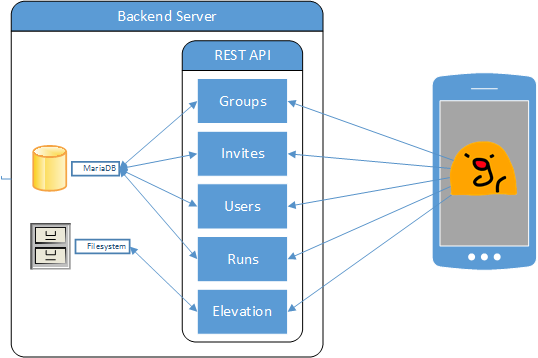
\includegraphics{abb/network_diagram_visio}
\caption{Kommunikation zwischen App und Backend-Server}
\end{figure}
Im folgenden erkläre ich die auf der Abbildung dargestellten Komponenten und warum diese für das Projekt gewählt wurden.
\subsection{Datenbank}
Als Datenbankverwaltungssystem  haben wir uns entschieden ``MariaDB'' zu nutzen. MariaDB ist das Pendant zu ``MySQL'', jedoch ist es schneller, sicherer und hat eine aktivere Community.
Beide Teammitglieder könne bereits auf längere Erfahrung in MySQL zurückgreifen. Die Arbeit mit MariaDB war aufgrund des weitgehend identischen Befehlssatzes sehr unkompliziert.
\subsection{REST API}
Um der App eine geeignete Schnittstelle zu Daten über das Internet bereitzustellen haben wir uns für eine REST API entschieden.
REST steht für ``Representational State Transfer'', einer stetig wachsenden 